% 05_dft_methods.tex -- Part 5, first-principles methods. Sources: research_monograph/chapters/M04_dft_theory.tex
% (Born-Oppenheimer, Kohn-Sham, PBE gap problem, HSE06, smearing), M04b_dft_numerics.tex (plane waves and N_pw table,
% PAW band counting and correction X1, SCF force error and correction V1, relaxation, slabs, dipole, two-step
% alignment), 13_dft_rev.tex (methods: data sets, convergence stage, k grids, slab recipe and symmetry, vacuum test,
% codes, GPU check, settings table incl. nbnd 190, band projections of the 1 nm W film), M10_w_and_vacancies.tex (W and
% H-L cell settings); evidence/FACT_REGISTRY.tsv (FACT-001, 002, 014, 019, 031, 042, 045);
% appendices/MG_corrections.tex (X1, X4, V1, V2); cern_htcondor/results/RESULTS_LOG.md (H-L settings: Gaussian 0.005 Ry,
% conv_thr 1e-8; 2 nm W film conv_thr 1e-8); ledger C035 (force-only check). Raw outputs read for checks:
% bulk_In2O3_protocol/vcrelax_ecut71_k3.out (nbnd 190), slab1r_final_cpu/scf.out (5 746 731 G-vectors),
% slab2_relax_c2/scf.out (82.10 GB), iwo_W8b/scf_k4.out and iwo_slab1_final_cpu/scf.out (printed MV occupations).
% MV convention: the slide uses the weight as Quantum ESPRESSO applies it, f = 1/2 erfc(u) + exp(-u^2)/sqrt(2 pi),
% u = (eps - mu)/sigma + 1/sqrt2, which reproduces every printed occupation of the W cells to 3e-4 (max printed 1.0738,
% none negative). Monograph eq. mono-dft-mv and the M04b key result ("MV weights can be negative") give the mirror image
% 1 - f(-x) and are flagged for an erratum; the slide does not repeat them.
% Figures: tools/fig_05_dft_methods.py (data: qe_workflow/analysis_2026-10-13_full/out/f01_bulk_convergence.json,
% f03_bulk_alignment.json, cern_htcondor/results/slab2_relax_c2/slab2_relax_c2_avg.dat, iwo_W8b/scf_k4.out).
% Blind rules: only protocol facts and force-only checks (C035) of the amorphous campaign appear; no electronic quantity
% of any amorphous cell.
% Note: frame bodies start with a command, never with a brace group (beamer would read a subtitle).
\providecommand{\fiveVV}{\bar{\bar{V}}}
% denser slides: footnotesize bullets, local to the frame in which it is called
\providecommand{\fivedense}{\setbeamerfont{itemize/enumerate body}{size=\footnotesize}%
  \setbeamerfont{itemize/enumerate subbody}{size=\footnotesize}}
% pull the frame body up to the title rule (frames are top-aligned, as in sections 02, 04, 10, 12-14)
\providecommand{\fiveTop}{\vspace{-2.5mm}}
% evidence label inside a \src line (inherits the \tiny grey source text instead of the larger \lab size)
\providecommand{\fivesrclab}[1]{[\textsc{\MakeLowercase{#1}}]}

\partslide{Part 5}{First-principles methods}

% ---------------------------------------------------------------------------------------------------------------------
\begin{frame}[t]{PBE gives the geometries; only gap differences are trusted}
  \fivedense\fiveTop
  \begin{columns}[T,onlytextwidth]
    \begin{column}{0.50\textwidth}
      \begingroup\footnotesize\textbf{Kohn--Sham DFT and the gap}\srefs{Hohenberg1964,Kohn1965,PerdewLevy1983,ShamSchluter1983}\par\endgroup
      \vspace{-3mm}
      \begingroup\footnotesize
      \begin{gather*}
        \Big[-\tfrac12\nabla^2 + v_{\mathrm{ext}} + v_{\mathrm{H}}[n] + v_{\mathrm{xc}}[n]\Big]\psi_j = \varepsilon_j\psi_j ,
        \quad n = \textstyle\sum_j f_j|\psi_j|^2 \\
        \Eg = \Eg^{\mathrm{KS}} + \Delta_{\mathrm{xc}}, \qquad \Delta_{\mathrm{xc}} = 0 \text{ in PBE}
      \end{gather*}\par\endgroup
      \vspace{-1.5mm}
      \begingroup\scriptsize\color{inkgrey}Hartree units. $v_{\mathrm{ext}}, v_{\mathrm{H}}, v_{\mathrm{xc}}$: nuclear,
        Hartree and exchange--correlation potentials; $f_j$: occupations; $\Delta_{\mathrm{xc}}$: jump of the exact
        $v_{\mathrm{xc}}$ at integer electron number.\par\endgroup
      \vspace{1mm}
      \begingroup\footnotesize Born--Oppenheimer, static lattice\sref{Born1927}: fixed nuclei; corrections in powers
        of $\kappa = (m_e/M)^{1/4}$, 0.076 (O) and 0.047 (In) \lab{derived}: vibrations at order $\kappa^2$,
        non-adiabatic terms higher (not estimated).\par\endgroup
    \end{column}
    \begin{column}{0.46\textwidth}
      \begin{itemize}
        \item PBE\sref{Perdew1996} for all relaxations and production runs. Bulk gap 0.8887\,eV \lab{computed};
          measured 2.7--2.9\,eV\srefs{Walsh2008,Irmscher2014}.
        \item HSE06\srefs{Heyd2003,Heyd2006,Krukau2006}: a fraction $\alpha = 0.25$ of the short-range exchange is
          exact, $\omega = 0.106$\,bohr$^{-1}$; fixed PBE geometry. Bulk gap 2.108\,eV (norm-conserving,
          $\Gamma$-only $q$; 41.8\,meV lower with $3\times3\times3$ $q$) \lab{computed}.
        \item Not included: zero-point renormalisation, spin--orbit coupling, spin polarisation (production
          runs) \lab{assumed}.
      \end{itemize}
    \end{column}
  \end{columns}
  \takeaway{No absolute PBE gap is used; only film-minus-bulk shifts, checked with HSE06 at 1\,nm.}
\end{frame}

% ---------------------------------------------------------------------------------------------------------------------
\begin{frame}[t]{A 71/568\,Ry basis met the criteria fixed before the runs}
  \fivedense\fiveTop
  \begin{columns}[T,onlytextwidth]
    \begin{column}{0.45\textwidth}
      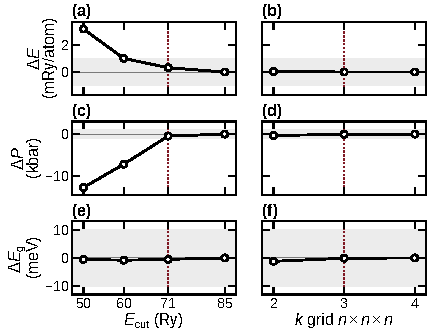
\includegraphics[width=0.93\linewidth]{05_convergence}
      \src{Bulk \InO{} (40-atom primitive cell at the experimental $a = 10.117$\,\AA{}), PAW-PBE: change against
        85\,Ry (left) and 4$\times$4$\times$4 (right). Grey: criteria; dotted: settings used (71\,Ry,
        3$\times$3$\times$3). This work \fivesrclab{computed}.}
    \end{column}
    \begin{column}{0.51\textwidth}
      \begin{itemize}
        \item Criteria (protocol of 26 Sep 2026): the next step may change the energy by $<1$\,mRy/atom, the pressure
          by $<1$\,kbar, the gap by $<10$\,meV.
        \item 71\,Ry is the lowest cutoff that passes: 0.32\,mRy/atom, 0.47\,kbar and 0.5\,meV against 85\,Ry
          \lab{computed}. PAW density cutoff: $8E_{\mathrm{cut}} = 568$\,Ry.
        \item Monkhorst--Pack grids\sref{Monkhorst1976}: 2$\times$2$\times$2 already passes; used: 3$\times$3$\times$3
          (bulk), 3$\times$3$\times$1 (slabs), 4$\times$4$\times$4 (80-atom W and H-L single points).
        \item Quantum ESPRESSO 7.5 on CPUs\srefs{Giannozzi2009,Giannozzi2017}, NVIDIA GPU build
          7.3.1\sref[NGC container \texttt{hpc/quantum\_espresso:qe-7.3.1}]{NvidiaQE}: the same input gives energies
          $5\times10^{-7}$\,Ry apart \lab{computed}.
      \end{itemize}
    \end{column}
  \end{columns}
\end{frame}

% ---------------------------------------------------------------------------------------------------------------------
\begin{frame}[t]{Plane-wave counts follow the volume law to within 0.15\,\%}
  \fivedense\fiveTop
  \begin{columns}[T,onlytextwidth]
    \begin{column}{0.57\textwidth}
      \vspace*{-0.5\abovedisplayskip}
      \begingroup\footnotesize
      \[
        N_{\mathrm{pw}} \approx \frac{4\pi k_c^3/3}{(2\pi)^3/\Omega} = \frac{\Omega\,E_{\mathrm{cut}}^{3/2}}{6\pi^2},
        \qquad k_c = E_{\mathrm{cut}}^{1/2}
      \]\par\endgroup
      \vspace{-0.3mm}
      \begingroup\scriptsize\color{inkgrey}$\Omega$: cell volume (bohr$^3$); $E_{\mathrm{cut}}$ in Ry; plane waves with
        $|\mathbf{k}+\mathbf{G}|^2 \le E_{\mathrm{cut}}$; $N_b$: number of bands.\par\endgroup
      \vspace{2mm}
      \begingroup\scriptsize
      \renewcommand{\arraystretch}{1.1}\setlength{\tabcolsep}{5.5pt}
      \begin{tabular}{@{}l r r r r@{}}
        \toprule
        Cell (atoms) & $\Omega$ (bohr$^3$) & formula & printed & bands \\
        \midrule
        bulk In$_{16}$O$_{24}$ (40, primitive) & 3\,693.6 & 37\,315 & 37\,359 & 190 \\
        bulk In$_{31}$WO$_{48}$ (80) & 7\,387.2 & 74\,630 & 74\,653 & 424 \\
        1\,nm slab In$_{24}$O$_{48}$H$_{24}$ (96) & 25\,140.0 & 253\,982 & 253\,973 & 328 \\
        2\,nm slab In$_{56}$O$_{96}$H$_{24}$ (176) & 32\,429.2 & 327\,622 & 327\,585 & 680 \\
        \bottomrule
      \end{tabular}\par\endgroup
      \src{$E_{\mathrm{cut}} = 71$\,Ry. Printed: plane waves at $\Gamma$ in the \texttt{pw.x} output; bands:
        \texttt{nbnd} of the run. This work \fivesrclab{computed}.}
    \end{column}
    \begin{column}{0.39\textwidth}
      \begin{itemize}
        \item The density sphere at $8E_{\mathrm{cut}}$ holds $8^{3/2} \approx 22.6$ times more components: 5\,746\,731
          for the 1\,nm slab \lab{computed}.
        \item Work per SCF step grows as $N_b^2N_{\mathrm{pw}}$. From 1 to 2\,nm: bands 328 to 680, $N_{\mathrm{pw}}$
          $+29$\,\%, work $\times5.5$ \lab{derived}.
        \item 2\,nm wave functions at one $k$ point: $680\times327\,585\times16$\,B $= 3.6$\,GB \lab{derived};
          \texttt{pw.x} estimates 82\,GB per process for the single-process GPU relaxation \lab{computed}.
      \end{itemize}
    \end{column}
  \end{columns}
  \takeaway{The 176-atom film needed a large-memory GPU or a distributed CPU run.}
\end{frame}

% ---------------------------------------------------------------------------------------------------------------------
\begin{frame}[t]{A W cell has one valence band fewer than the pure cell}
  \fivedense\fiveTop
  \begin{columns}[T,onlytextwidth]
    \begin{column}{0.47\textwidth}
      \begingroup\footnotesize PAW\srefs{Bloechl1994,Kresse1999}, pslibrary 1.0.0 data sets\sref{DalCorso2014}\par\endgroup
      \vspace{0.5mm}
      \begingroup\scriptsize
      \renewcommand{\arraystretch}{1.0}
      \begin{tabular}{@{}l l r l@{}}
        \toprule
        & valence & $Z$ & bands below the gap \\
        \midrule
        In & 4d$^{10}$5s$^2$5p$^1$ & 13 & 5 (In 4d) \\
        W  & 5s$^2$5p$^6$5d$^4$6s$^2$ & 14 & 4 (W 5s, 5p) \\
        O  & 2s$^2$2p$^4$ & 6 & 4 (O 2s, 2p) \\
        H  & 1s$^1$ & 1 & none (O--H within O bands) \\
        \bottomrule
      \end{tabular}\par\endgroup
      \vspace{1.1mm}
      \begingroup\footnotesize\centering
        $N_{\mathrm{VB}} = 5n_{\mathrm{In}} + 4n_{\mathrm{W}} + 4n_{\mathrm{O}}, \qquad
        N_{\mathrm{ex}} = \textstyle\sum Z - 2N_{\mathrm{VB}}$\par\endgroup
      \vspace{0.9mm}
      \begingroup\scriptsize
      \renewcommand{\arraystretch}{1.0}
      \begin{tabular}{@{}l r r r@{}}
        \toprule
        cell & $\sum Z$ & $N_{\mathrm{VB}}$ & $N_{\mathrm{ex}}$ \\
        \midrule
        bulk In$_{32}$O$_{48}$ (80-atom conventional) & 704 & 352 & 0 \\
        bulk In$_{31}$WO$_{48}$ & 705 & 351 & 3 \\
        1\,nm In$_{24}$O$_{48}$H$_{24}$ & 624 & 312 & 0 \\
        1\,nm In$_{23}$WO$_{48}$H$_{24}$ & 625 & 311 & 3 \\
        \bottomrule
      \end{tabular}\par\endgroup
      \src{$Z$: valence charges of the data sets; $\sum Z$ as printed by \texttt{pw.x} \fivesrclab{computed};
        $N_{\mathrm{VB}}$, $N_{\mathrm{ex}}$ \fivesrclab{derived}.}
    \end{column}
    \begin{column}{0.49\textwidth}
      \centering
      \begin{tikzpicture}[x=1mm,y=1mm,line width=0.5pt,font=\scriptsize]
        \node[anchor=south] at (9.5,24.2) {1\,nm In$_{24}$O$_{48}$H$_{24}$};
        \node[anchor=south] at (50.5,24.2) {1\,nm In$_{23}$WO$_{48}$H$_{24}$};
        % pure cell
        \draw (0,0) rectangle (19,8.5);
        \node[align=center] at (9.5,4.25) {bands 1--312\\occupied};
        \draw (0,13) rectangle (19,24);
        \node[align=center] at (9.5,18.5) {bands 313--\\empty};
        % W cell
        \draw (33,0) rectangle (68,8.5);
        \node[align=center] at (50.5,4.25) {bands 1--311\\occupied (valence)};
        \draw (33,13) rectangle (68,24);
        \draw[rulegrey] (33,18.5) -- (68,18.5);
        \node at (50.5,15.75) {312: host CB bottom, 2\,e$^-$};
        \node at (50.5,21.25) {313: W-5d rich, $\approx$1\,e$^-$};
        \node[inkgrey] at (9.5,10.75) {gap};
        \node[inkgrey] at (50.5,10.75) {gap};
        % the misreading of 30 September
        \node[align=center,ntumaroon] (mis) at (26,4.25) {W cell:\\312 read\\as VB top};
        \draw[-{Stealth[length=1.6mm]},ntumaroon,line width=0.7pt] (mis.north) .. controls (26,12.5) and (27.5,15.75) .. (32.6,15.75);
      \end{tikzpicture}
      \vspace{1mm}
      \begin{itemize}
        \item At $\Gamma$: band 311 is O 2p, 313 has 56\,\% W 5d, resonant 1.22\,eV above the host band bottom in
          this film (2\,nm: 1.34\,eV; bulk: 1.76--1.80\,eV), at the computed filling of 3\,e per cell
          \lab{computed}.
      \end{itemize}
    \end{column}
  \end{columns}
  \takeaway{Reading band 312 as the VB top caused the 30 Sep ``W level below CB'' (correction X1).}
\end{frame}

% ---------------------------------------------------------------------------------------------------------------------
\begin{frame}[t]{Marzari--Vanderbilt weights exceed 1 below $\mu$: not occupations}
  \fivedense\fiveTop
  \begin{columns}[T,onlytextwidth]
    \begin{column}{0.42\textwidth}
      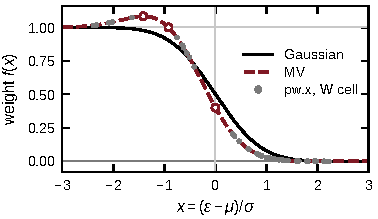
\includegraphics[width=\linewidth]{05_smearing}
      \src{MV as \texttt{pw.x} applies it: $f = \tfrac12\mathrm{erfc}(u) + e^{-u^2}\!/\sqrt{2\pi}$,
        $u = x + 1/\sqrt2$. Circles: 0.40, 1 and 1.083 at $x = 0$, $-0.92$, $-\sqrt2$ \fivesrclab{derived}. Dots: 51
        fractional weights printed by \texttt{pw.x} for a bulk W cell (largest 1.074), within $3\times10^{-4}$ of $f$
        \fivesrclab{computed}.}
    \end{column}
    \begin{column}{0.55\textwidth}
      \begin{itemize}
        \item W cells are metals: weights $f(x)$, $x = (\varepsilon-\mu)/\sigma$; $F = E - \sigma S$ is
          variational\sref{Mermin1965}.
        \item Gaussian $\tfrac12\mathrm{erfc}(x)$ stays in $[0,1]$. Marzari--Vanderbilt (MV)\sref{Marzari1999}: energy
          error $O(\sigma^3)$, but 0.40 at $\mu$ and 1.083 at $\sqrt2\sigma$ below $\mu$ (0.19\,eV at 0.01\,Ry)
          \lab{derived}.
        \item Counts near $\mu$ depend on $\sigma$ and $f$: the W-5d projections (0.09--0.43\,e \lab{computed}) are
          not a W charge.
      \end{itemize}
      \vspace{0.5mm}
      \begingroup\scriptsize
      \begin{tabular}{@{}r r l l@{}}
        \toprule
        $\sigma$ (Ry) & (meV) & $f$ & used for \\
        \midrule
        0.01 & 136 & MV & W cells (site study, films) \\
        0.005 & 68 & Gaussian & H-L cells, with and without W \\
        0.002 & 27 & Gaussian & H-L width check \\
        0.001 & 13.6 & Gaussian & amorphous reference finals \\
        \bottomrule
      \end{tabular}\par\endgroup
      \src{\texttt{pw.x} inputs; this work. For comparison, $\kT = 25.85$\,meV at 300\,K.}
    \end{column}
  \end{columns}
  \takeaway{Shallow occupations need Gaussian smearing well below the energy differences.}
\end{frame}

% ---------------------------------------------------------------------------------------------------------------------
\begin{frame}[t]{Slab band edges are placed on the bulk scale in two steps}
  \fivedense\fiveTop\toggletrue{blx@useprefix}% print "Van de Walle" in the footnote (local to this frame)
  \begin{columns}[T,onlytextwidth]
    \begin{column}{0.42\textwidth}
      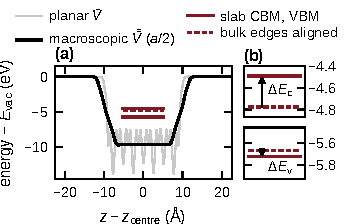
\includegraphics[width=\linewidth]{05_alignment}
      \src{Relaxed 2\,nm (001) slab, PAW-PBE. (a) Ionic plus Hartree potential, planar ($\bar V$) and macroscopic
        ($\fiveVV$) averages; solid: slab edges; dashed: bulk edges via the interior $\fiveVV$. (b) Edges magnified
        (0.47\,eV windows). This work \fivesrclab{computed}.}
    \end{column}
    \begin{column}{0.55\textwidth}
      \begin{itemize}
        \item (001) films, H on surface O that lost In, 25\,\AA{} vacuum\sref[p.~21542]{Lin2022}; 15--35\,\AA{}
          moves EA, IP by $\le 0.1$\,meV \lab{computed}.
        \item Two-step alignment\srefs{VandeWalle1987,Baldereschi1988}; $\fiveVV$: $\bar V$ averaged over $a/2$:
          \[ \dEc = \big(E^{\mathrm{slab}}_{\mathrm{CBM}} - \fiveVV^{\,\mathrm{slab}}_{\mathrm{int}}\big)
                  - \big(E^{\mathrm{bulk}}_{\mathrm{CBM}} - \fiveVV^{\,\mathrm{bulk}}\big) \]
          2\,nm: interior flat within 8\,meV; $\dEc = +0.281$\,eV, $\dEv = -0.054$\,eV \lab{computed}.
        \item 1, 2\,nm: Pcca maps one face onto the other, no dipole \lab{computed}. A sawtooth dipole
          correction\srefs{Neugebauer1992,Bengtsson1999} puts the step in the vacuum; the polar 0.695\,nm film ran
          without it: step 0.44\,V (0.35--0.37\,V if the ramp spans only the vacuum), $\le 0.095$\,eV across the
          film; its effect on the gap is untested \lab{derived}.
      \end{itemize}
    \end{column}
  \end{columns}
  \takeaway{The polar 0.695\,nm film stays out of new primary $\dEc$ fits (correction X4).}
\end{frame}

% ---------------------------------------------------------------------------------------------------------------------
\begin{frame}[t]{SCF force noise is 15 times below the $10^{-3}$\,Ry/bohr threshold}
  \fivedense\fiveTop
  \vspace{-1.8mm}
  \begingroup\scriptsize
  \renewcommand{\arraystretch}{0.95}
  \begin{tabularx}{\textwidth}{@{}l l c c c X@{}}
    \toprule
    Structures & calculation & forces (Ry/bohr) & energy (Ry) & pressure (kbar) & cell degrees of freedom \\
    \midrule
    bulk \InO{} & vc-relax & $10^{-4}$ & $10^{-5}$ & 0.2 & BFGS, all lattice vectors \\
    slabs & vc-relax & $10^{-3}$ & $10^{-4}$ & 0.5 & BFGS, in-plane vectors only \\
    W and H-L cells & relax & $10^{-3}$ & $10^{-4}$ & -- & fixed \\
    \bottomrule
  \end{tabularx}\par\endgroup
  \src{Stopping thresholds. Ions and cell by BFGS, not damped dynamics (correction V2); SCF threshold $10^{-9}$\,Ry ($10^{-8}$\,Ry: metallic
    2\,nm W film, six H-L cells). \texttt{pw.x} inputs; this work.}
  \vspace{-1.5mm}
  \begin{columns}[T,onlytextwidth]
    \begin{column}{0.49\textwidth}
      \begin{itemize}
        \item BFGS\sref{Billeter2003} steps along $-\mathbf{H}^{-1}\nabla E$ ($\mathbf{H}$: approximate Hessian).
          Bulk: 11 steps to $a = 10.306$\,\AA, 1.87\,\% above experiment\sref{Marezio1966} \lab{computed}.
        \item The criterion is per component: the relaxed 1\,nm slab has a norm of $6.1\times10^{-3}$\,Ry/bohr over
          288 components, typically $3.6\times10^{-4}$ \lab{derived}.
        \item \texttt{pw.x} writes coordinates even after a failed BFGS run; amorphous chains need ``bfgs
          converged'' (amendment A19).
      \end{itemize}
    \end{column}
    \begin{column}{0.49\textwidth}
      \begin{itemize}
        \item SCF error $\delta n$: energy error second order, force error first order:
          $\delta F \propto \sqrt{\smash[b]{\texttt{conv\_thr}}}$.
        \item Amorphous 1.0\,nm cell, 134 atoms (force-only check C035), \texttt{conv\_thr} $10^{-7}$\,Ry: SCF force
          correction (norm) $1.3\times10^{-3}$\,Ry/bohr \lab{computed}.
        \item Per component: $1.3\times10^{-3}/\sqrt{402} \approx 6\times10^{-5}$\,Ry/bohr, 15 times below
          $10^{-3}$\,Ry/bohr (correction V1) \lab{derived}.
      \end{itemize}
    \end{column}
  \end{columns}
  \takeaway{Force differences below $10^{-4}$\,Ry/bohr per component need tighter SCF thresholds.}
\end{frame}
